\DocumentMetadata{
  lang=en,
  pdfstandard=ua-2,
  pdfstandard=a-4f,
  tagging=on
}
% Options for packages loaded elsewhere
\PassOptionsToPackage{unicode}{hyperref}
\PassOptionsToPackage{hyphens}{url}
\documentclass[
]{article}
\usepackage{xcolor}
\usepackage{amsmath,amssymb}
\setcounter{secnumdepth}{5}
\usepackage{iftex}
\ifPDFTeX
  \usepackage[T1]{fontenc}
  \usepackage[utf8]{inputenc}
  \usepackage{textcomp} % provide euro and other symbols
\else % if luatex or xetex
  \usepackage{unicode-math} % this also loads fontspec
  \defaultfontfeatures{Scale=MatchLowercase}
  \defaultfontfeatures[\rmfamily]{Ligatures=TeX,Scale=1}
\fi
\usepackage{lmodern}
\ifPDFTeX\else
  % xetex/luatex font selection
\fi
% Use upquote if available, for straight quotes in verbatim environments
\IfFileExists{upquote.sty}{\usepackage{upquote}}{}
\IfFileExists{microtype.sty}{% use microtype if available
  \usepackage[]{microtype}
  \UseMicrotypeSet[protrusion]{basicmath} % disable protrusion for tt fonts
}{}
\makeatletter
\@ifundefined{KOMAClassName}{% if non-KOMA class
  \IfFileExists{parskip.sty}{%
    \usepackage{parskip}
  }{% else
    \setlength{\parindent}{0pt}
    \setlength{\parskip}{6pt plus 2pt minus 1pt}}
}{% if KOMA class
  \KOMAoptions{parskip=half}}
\makeatother
\setlength{\emergencystretch}{3em} % prevent overfull lines
\providecommand{\tightlist}{%
  \setlength{\itemsep}{0pt}\setlength{\parskip}{0pt}}
\sloppy
\setlength{\emergencystretch}{3em}
\usepackage{booktabs}
\usepackage{caption}
\usepackage{float}
\usepackage{tabularx}
\usepackage{tikz}
\usepackage{flowchart}
\usetikzlibrary{arrows.meta,fit,positioning}
\usepackage{bookmark}
\IfFileExists{xurl.sty}{\usepackage{xurl}}{} % add URL line breaks if available
\urlstyle{same}
\hypersetup{
  pdftitle={FOI-O: Reusable ontology and verification infrastructure for Freedom of Information systems},
  pdfauthor={Dylan A Mordaunt},
  hidelinks,
  pdfcreator={LaTeX via pandoc}}

\title{FOI-O: Reusable ontology and verification infrastructure for
Freedom of Information systems}
\author{Dylan A Mordaunt\textsuperscript{1,2,3}}
\date{2026-07-02}

\begin{document}
\maketitle
\begin{abstract}
Public official-information request records contain process signals.
They can support research, workflow review, and human-supervised agent
help. Yet they also mix observed correspondence, platform states,
inferred events, and legal outcomes. FOI-O is a reusable process
ontology and verification infrastructure for Freedom of Information
administration. It uses the New Zealand Official Information Act as the
first worked jurisdictional example. The Act is a starting point, not
the limit of the model. Key terms and abbreviations are defined after
the references. The aim is to create reusable resources for comparing,
checking, and improving public-information request processes across
jurisdictions. FOI-O models the request record first. Request profiles,
observed correspondence events, controlled vocabularies, and provenance
make visible what was seen and how it was changed. It then adds review
queues, release metadata, and bounded agent contracts. Human
certification of legally meaningful outcomes stays outside autonomous
tooling. The repository provides JavaScript Object Notation (JSON)
Schema contracts and Python data models for operational checks. It also
provides Simple Knowledge Organization System (SKOS) vocabularies, Web
Ontology Language (OWL), Resource Description Framework (RDF), and
Shapes Constraint Language (SHACL) assets for semantic review. These are
supported by deterministic examples, release metadata, quality gates,
and tests. This article describes the motivation, architecture,
ontology-development method, validation evidence, and implementation
boundaries. The project is not legal advice, is not an official
government publication, and does not certify release, refusal,
redaction, charging, extension, transfer, complaint, or publication
outcomes.
\end{abstract}

\textsuperscript{1} Faculty of Health, Education and Psychology,
Victoria University of Wellington. \textsuperscript{2} College of
Medicine and Public Health, Flinders University. \textsuperscript{3}
Centre for Health Policy, The University of Melbourne.

\textbf{Keywords:} Freedom of Information; Official Information Act;
ontology engineering; process mining; public administration; legal
informatics; agent safety.

\section{Introduction}\label{introduction}

Freedom of Information (FOI; see the
\hyperlink{tab-abbreviations}{abbreviations table}) administration has
many process steps. This is true across many legal systems. Yet the
process is often hard to compare across institutions and jurisdictions.
In this article, FOI refers to legal and administrative systems that
allow people to request information from public bodies. A single request
usually begins with intake: the request is received, registered,
acknowledged, and sometimes clarified or transferred to another body. It
then moves into decision-making, where deadlines, extensions, searches,
consultations, charges, redactions, releases, and refusals may need to
be recorded {[}1-3{]}. After the decision, the same request may still
matter for complaints, publication, disclosure logs, performance
statistics, and later reporting. Practitioners know these steps well.
They are not always recorded in a consistent machine-readable form.
Evidence may be spread across email, case-management tools, public
request platforms, disclosure logs, spreadsheets, attachments, and
statistical reports. As a result, the same process event can be visible
as a message in one system, a platform state in another, and a reporting
category in a third.

This makes FOI administration a useful but demanding target for process
modelling. Public request records show how requests move through real
administrative workflows. They can show when a request was made. They
can show whether an agency acknowledged it, sought clarification,
changed an apparent due date, released information, or faced a public
complaint. Public platforms such as FYI.org.nz (FYI; see the
\hyperlink{tab-abbreviations}{abbreviations table}) are especially
useful because they make parts of the request history visible outside
the agency. Even so, these records are platform-mediated evidence. They
are not agency systems of record. They can be incomplete, delayed,
duplicated, redacted, or unclear. A platform label may not match the
legal status of a request. A message timestamp may not be the statutory
date that matters. A visible attachment may not be the full agency
decision. Any reusable FOI data model therefore needs to preserve what
was observed while clearly marking what was inferred {[}6-13{]}.

The problem is not only technical. FOI systems support democratic
accountability, public-sector learning, journalism, research, and
individual rights. When the process is hard to inspect, it is harder to
compare agency practice. It is also harder to explain delays, assess
reporting, or see where request handling could improve. A global
resource for FOI processes therefore needs to be clear to more than
software developers. It should describe the journey of a request in
words that policy analysts, lawyers, researchers, civic technologists,
and public officials can examine. It must also be precise enough for
machines to check examples, detect missing evidence, and support
reproducible analysis. Recent public-governance evidence supports this
need. OECD trust-survey work links trust in public institutions to
transparency, responsiveness, integrity, and evidence-informed
decisions. Open-government measurement frameworks also treat access to
information as a core part of accountable government {[}10,13,14{]}.

This also fits an older idea in democratic theory. Popper's open society
concept stresses public criticism, correction, and the ability to
challenge official power {[}8{]}. FOI gives that idea an administrative
form. It lets people ask what government has done, inspect the records
that support decisions, and test public claims against evidence.
Computation can help this work when it sorts, links, checks, and
explains records. It supports open government best when it widens
scrutiny without replacing human judgement or public accountability.

The same distinction matters for agent-facing systems. Modern
extraction, retrieval, summary, and validation tools can help organise
FOI material. They can also create risk. A candidate signal may be
mistaken for an official outcome. For example, an automated system might
identify a message that looks like an extension notice. It might also
identify a document that appears to contain released information. That
does not mean the system can certify whether the extension, release,
refusal, redaction, charge, transfer, or complaint outcome was lawful or
final. FOI-O addresses this risk by treating public FOI workflow data as
evidence for review, not as autonomous legal decision-making. Its core
distinction is between observed evidence, candidate interpretation, and
human-certified outcome. Agents may help with routing, summary, event
extraction, evidence checks, and review preparation. Authorised humans
remain responsible for legally meaningful decisions {[}23-25{]}.

The New Zealand Official Information Act (OIA; see the
\hyperlink{tab-abbreviations}{abbreviations table}) is used as the first
worked jurisdictional example. This starting point is deliberate, but it
is not limiting. New Zealand provides a concrete legal and
administrative setting that the author understands. FYI also provides
public request material that can test a practical model {[}1-5{]}. The
broader goal is international. FOI regimes differ in deadlines,
exemptions, appeal paths, proactive publication practice, reporting
categories, and institutional culture. They also share recurring process
problems. Requests are received, clarified, routed, answered, refused,
extended, published, challenged, and counted. A reusable ontology should
make those common structures visible. It should also allow local rules
and terms to be added later.

FOI-O therefore aims to provide comparative infrastructure, not a New
Zealand-only artefact. It can support future resources for comparing FOI
processes across countries. It can help identify good practice, document
weak process evidence, and show how a request moved from source record
to candidate event and then to any human-certified status. The current
contribution is a bounded, reproducible methods package. It is not a
live public-service system. It defines an auditable data model, semantic
layer, validation gates, local examples, repository architecture,
process architecture, data-model diagrams, release metadata, and tests.
These can be inspected without live credentials or private request
content. Together, they show the boundary between repository-local proof
and future external validation.

The article is organised as follows. The Methods section states the
design principles, repository architecture, ontology-development
protocol, data model, and human-certification boundary. The Results
section describes what the current repository implements and validates.
The Discussion explains why this bounded architecture matters for
comparative FOI research and safer agent-assisted public administration
{[}23-25{]}.

\section{Methods}\label{methods}

\subsection{Design Principles}\label{design-principles}

FOI-O was developed around five design principles. The first two protect
the evidence record. Source evidence is kept before interpretation. This
means that observed labels, timestamps, correspondence records, platform
states, and attachment references are retained before they are mapped to
normalised process concepts. Observation is also kept separate from
certification. An extracted event may be useful for review, but it is
not treated as a final legal or administrative outcome unless a
human-authorised record supports that status.

The next two principles protect clarity and safety. Semantics remain
inspectable because schemas, controlled vocabularies, ontology files,
validation rules, mappings, examples, and tests are kept as reviewable
artefacts. They are not hidden inside a model or prompt. The system
fails closed around legal outcomes. When evidence is missing, unclear,
or generated by an automated component, the output is framed as a
candidate signal for review rather than a certified decision. The final
principle concerns proof. Local proof is preferred over aspirational
claims. Repository tests, examples, quality gates, and generated
metadata define what the package can currently show. Live services and
jurisdictional adoption remain external gates.

The design principles and implementation consequences are summarised in
\hyperlink{tab-design-principles}{Table 1}.

\begin{table}[H]
\small
\hypertarget{tab-design-principles}{}
\begin{center}\small\textbf{Table 1: Design principles used to develop the FOI-O methods package. Abbreviations: FOI, Freedom of Information.}\end{center}
\begin{tabularx}{\linewidth}{>{\raggedright\arraybackslash}p{0.34\linewidth}X}
\toprule
Principle & Implementation consequence \\
\midrule
Preserve source evidence & Keep observed labels, timestamps, and evidence before mapping to normalised states. \\
Separate observation from certification & Mark candidate events as reviewable signals, not final legal outcomes. \\
Keep semantics inspectable & Commit JSON Schema, SKOS, OWL, RDF, SHACL, mappings, and examples as reproducible artefacts. \\
Fail closed around legal outcomes & Reject autonomous certification of decision-like outcomes. \\
Prefer local proof & Use tests, examples, and validation commands to define what the repository can prove. \\
\bottomrule
\end{tabularx}
\end{table}

\subsection{Repository Architecture}\label{repository-architecture}

The architecture follows a source, archive, semantic, agent, and
evaluation layering pattern. Source request records and archive
manifests are preserved upstream. FOI-O maps those records into request
profiles, event streams, and controlled vocabularies. It also maps them
into Resource Description Framework (RDF; see the
\hyperlink{tab-abbreviations}{abbreviations table}) and Shapes
Constraint Language (SHACL; see the
\hyperlink{tab-abbreviations}{abbreviations table}) artefacts, plus
bounded agent resources {[}15-20{]}.

\hyperlink{fig-repository-architecture}{Figure 2} shows the
repository-level architecture, while
\hyperlink{fig-process-architecture}{Figure 3} shows the process flow
through validation and the human-certification boundary.

\begin{figure}[H]
\centering
\resizebox{\linewidth}{!}{%
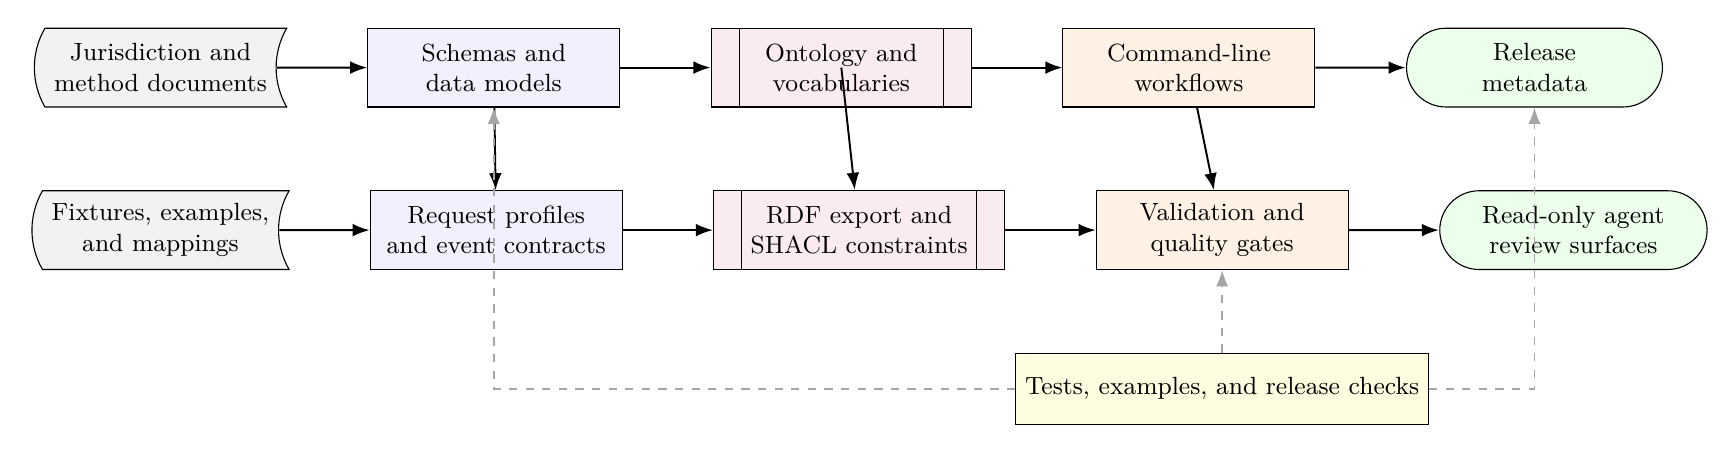
\begin{tikzpicture}[
  node distance=1.05cm and 1.15cm,
  every node/.style={font=\small, align=center},
  flow/.style={-Latex, line width=0.7pt},
  support/.style={-Latex, dashed, line width=0.65pt, draw=gray!70},
  asset/.style={storage, draw, minimum width=3.2cm, minimum height=1.0cm, fill=gray!10},
  contract/.style={process, draw, minimum width=3.2cm, minimum height=1.0cm, fill=blue!6},
  semantic/.style={predproc, draw, minimum width=3.3cm, minimum height=1.0cm, fill=purple!8},
  runtime/.style={process, draw, minimum width=3.2cm, minimum height=1.0cm, fill=orange!10},
  output/.style={terminal, draw, minimum width=3.25cm, minimum height=1.0cm, fill=green!8},
  qa/.style={process, draw, minimum width=3.45cm, minimum height=0.9cm, fill=yellow!12}
]
\node[asset] (docs) {Jurisdiction and\\method documents};
\node[asset, below=of docs] (examples) {Fixtures, examples,\\and mappings};
\node[contract, right=of docs] (schemas) {Schemas and\\data models};
\node[contract, right=of examples] (events) {Request profiles\\and event contracts};
\node[semantic, right=of schemas] (ontology) {Ontology and\\vocabularies};
\node[semantic, right=of events] (shacl) {RDF export and\\SHACL constraints};
\node[runtime, right=of ontology] (cli) {Command-line\\workflows};
\node[runtime, right=of shacl] (quality) {Validation and\\quality gates};
\node[output, right=of cli] (publication) {Release\\metadata};
\node[output, right=of quality] (agent) {Read-only agent\\review surfaces};
\node[qa, below=1.05cm of quality] (tests) {Tests, examples, and release checks};

\draw[flow] (docs) -- (schemas);
\draw[flow] (examples) -- (events);
\draw[flow] (schemas) -- (ontology);
\draw[flow] (events) -- (shacl);
\draw[flow] (ontology) -- (cli);
\draw[flow] (shacl) -- (quality);
\draw[flow] (cli) -- (publication);
\draw[flow] (quality) -- (agent);
\draw[flow] (schemas) -- (events);
\draw[flow] (ontology) -- (shacl);
\draw[flow] (cli) -- (quality);
\draw[support] (tests) -| (schemas.south);
\draw[support] (tests) -- (quality);
\draw[support] (tests) -| (publication.south);
\end{tikzpicture}%
}
\hypertarget{fig-repository-architecture}{}
\begin{center}\small\textbf{Figure 2: FOI-O repository architecture. The repository is organised as reviewable documents and fixtures, machine-readable contracts, semantic assets, runtime workflows, release metadata, read-only agent surfaces, and tests that bind the layers together. Abbreviations: FOI-O, Freedom of Information Ontology; RDF, Resource Description Framework; SHACL, Shapes Constraint Language.}\end{center}
\end{figure}

\begin{figure}[H]
\centering
\resizebox{\linewidth}{!}{%
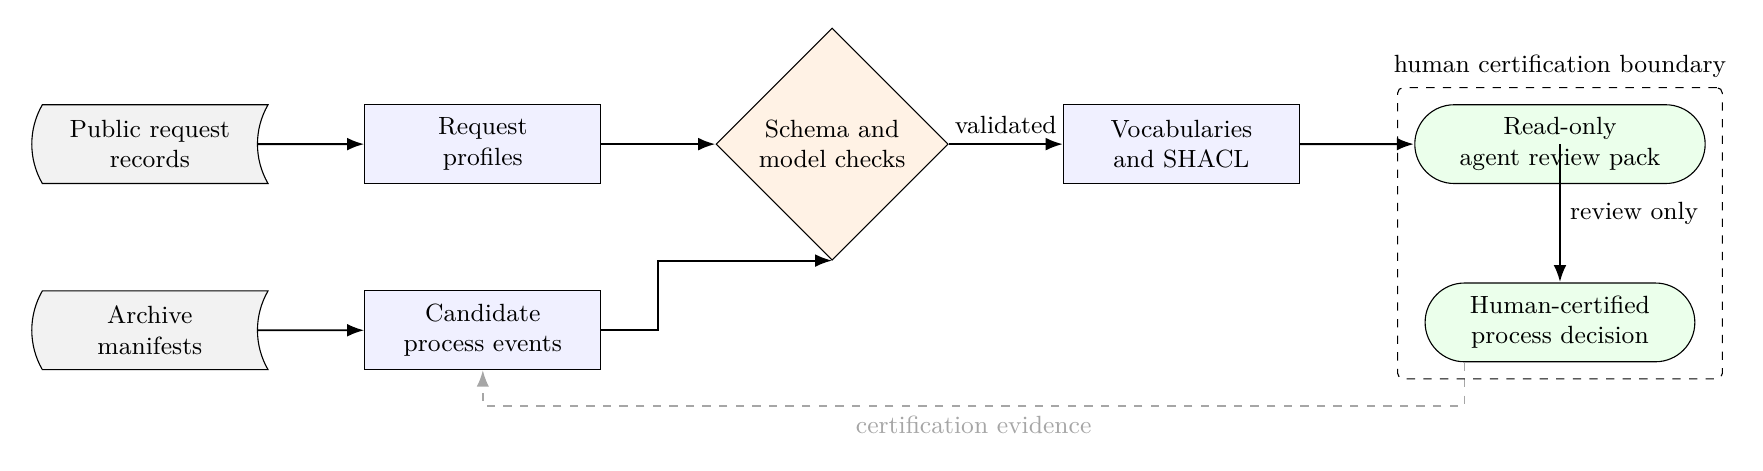
\begin{tikzpicture}[
  node distance=1.35cm and 1.35cm,
  every node/.style={font=\small, align=center},
  flow/.style={-Latex, line width=0.7pt},
  feedback/.style={-Latex, dashed, line width=0.65pt, draw=gray!70},
  store/.style={storage, draw, minimum width=3.0cm, minimum height=1.0cm, fill=gray!10},
  proc/.style={process, draw, minimum width=3.0cm, minimum height=1.0cm, fill=blue!6},
  check/.style={decision, draw, aspect=2, minimum width=2.6cm, minimum height=1.2cm, fill=orange!10},
  guard/.style={terminal, draw, minimum width=3.4cm, minimum height=1.0cm, fill=green!8},
  boundary/.style={draw, dashed, rounded corners=2pt, inner sep=6pt}
]
\node[store] (source) {Public request\\records};
\node[store, below=of source] (archive) {Archive\\manifests};
\node[proc, right=of source] (profile) {Request\\profiles};
\node[proc, right=of archive] (events) {Candidate\\process events};
\node[check, right=1.45cm of profile] (validation) {Schema and\\model checks};
\node[proc, right=1.45cm of validation] (semantic) {Vocabularies\\and SHACL};
\node[guard, right=1.45cm of semantic] (agent) {Read-only\\agent review pack};
\node[guard, below=1.25cm of agent] (human) {Human-certified\\process decision};

\draw[flow] (source) -- (profile);
\draw[flow] (archive) -- (events);
\draw[flow] (profile) -- (validation);
\draw[flow] (events.east) -- ++(0.72cm,0) |- (validation.south);
\draw[flow] (validation) -- node[above, midway]{validated} (semantic);
\draw[flow] (semantic) -- (agent);
\draw[flow] (agent) -- node[right]{review only} (human);
\draw[feedback] (human.south west) -- ++(0,-0.55cm) -| node[below,pos=0.25, text=gray!70]{certification evidence} (events.south);

\node[boundary, fit=(agent) (human), label={[font=\small]above:human certification boundary}] {};
\end{tikzpicture}%
}
\hypertarget{fig-process-architecture}{}
\begin{center}\small\textbf{Figure 3: FOI-O process architecture. Public request platforms and archive manifests are transformed into request profiles and candidate process events, checked through schema and model validation, aligned with semantic vocabularies and constraints, and packaged for read-only agent review before any human-certified process decision. Abbreviations: FOI-O, Freedom of Information Ontology; SHACL, Shapes Constraint Language.}\end{center}
\end{figure}

The Python control plane owns schema validation, FYI manifest
normalisation, event extraction, quality gates, reporting profiles, RDF
export, SHACL validation, release metadata, and command-line workflows.
Optional surfaces add runtime capability when installed. They do not
define the core proof. Deterministic Python paths and fixtures remain
the reproducibility base. FastMCP could expose read-only tool contracts
to agents. pySHACL can validate RDF graphs against SHACL constraints.
LanceDB is an embedded vector database. It could support local semantic
retrieval over request text, evidence chunks, and ontology terms. Mojo
and Modular MAX are being explored as local high-performance inference
tools. They could later support bounded extraction or embedding
workflows. They are not required for the current package. The present
evidence depends on portable schemas, examples, semantic assets, and
Python tests, not on specialised runtimes, hardware, or model-serving
installs.

\subsection{Ontology Development
Protocol}\label{ontology-development-protocol}

The ontology-development protocol uses repository evidence as the source
of truth. The first step is scoping. FOI-O identifies process concepts
from FOI request workflows, FYI/Alaveteli source states,
statutory-process concepts, release metadata, and reporting needs. New
Zealand OIA material is used as the first worked example. This produces
a practical concept inventory before the project attempts richer formal
modelling.

The second step is operational encoding. The project encodes the minimum
contracts as JavaScript Object Notation (JSON; see the
\hyperlink{tab-abbreviations}{abbreviations table}) Schemas and Pydantic
models before adding semantic alignments. This makes examples and
command outputs testable early. Controlled vocabularies are then defined
for request states, event types, assertion status, and agent boundaries
using the Simple Knowledge Organization System (SKOS; see the
\hyperlink{tab-abbreviations}{abbreviations table}).

The third step is semantic alignment. Event and evidence concepts are
aligned with the Provenance Ontology (PROV-O; see the
\hyperlink{tab-abbreviations}{abbreviations table}). This keeps
transformations and sources traceable. Dataset and publication concepts
are aligned with the Data Catalog Vocabulary (DCAT; see the
\hyperlink{tab-abbreviations}{abbreviations table}). Rights and policy
concepts use the Open Digital Rights Language (ODRL; see the
\hyperlink{tab-abbreviations}{abbreviations table}), SKOS, and
legal-document references where appropriate {[}15-20{]}. Safety and
consistency constraints are expressed in SHACL. The resulting examples
and code paths are validated through tests, release-readiness checks,
and machine-readable release metadata.

The core event contract defines observed and candidate process events.
Semantic constraints define how machine-readable process statements are
checked before they are used in reports, review packs, or agent-facing
workflows.

\subsection{Data Model}\label{data-model}

The model is organised in three groups. The request and event core
describes request profiles, process events, evidence references,
assertion status, provenance, generator metadata, and
human-certification metadata. This is the part of the model that records
what happened, where the evidence came from, and how strongly a process
statement can be asserted.

The review and governance layer describes agent actions, review tasks,
ledgers, chunks, and risk assessments. These records show how candidate
outputs were generated and reviewed, without turning them into legal
determinations. The reporting and release layer describes reporting
metrics and release metadata. Candidate process events can support
triage and review, but they are not promoted to certified outcomes
unless an authorised human record supplies the certification evidence.

\hyperlink{fig-data-model}{Figure 4} shows the main data-model
relationships, and \hyperlink{tab-data-model-surfaces}{Table 5}
summarises the corresponding model surfaces.

\begin{figure}[H]
\centering
\resizebox{\linewidth}{!}{%
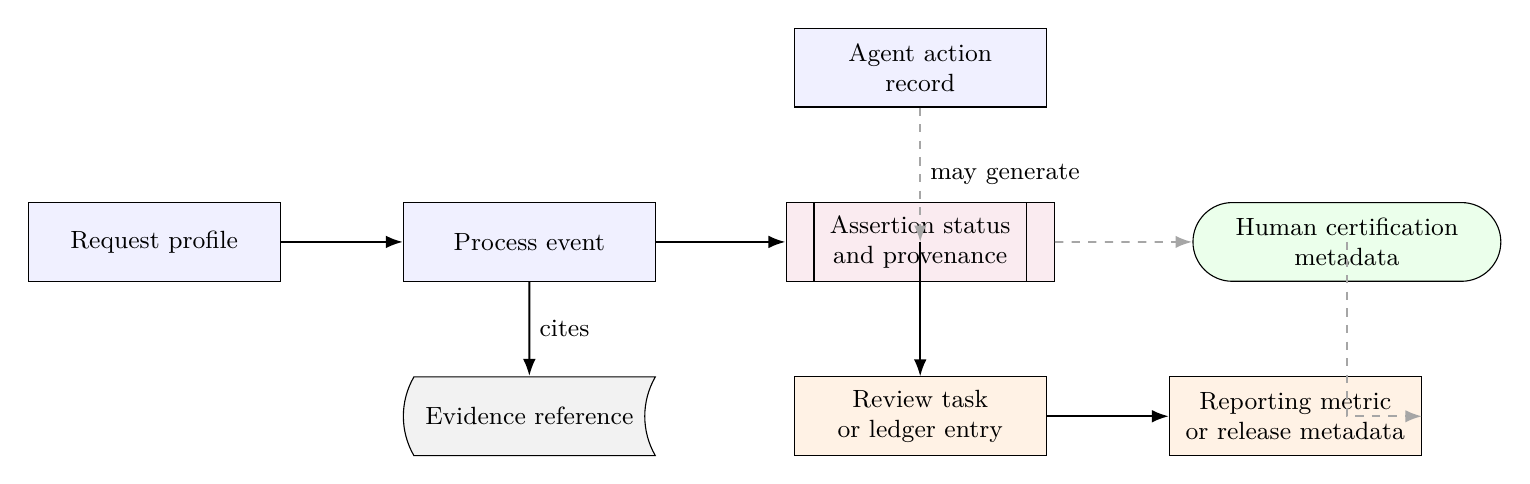
\begin{tikzpicture}[
  node distance=1.2cm and 1.55cm,
  every node/.style={font=\small, align=center},
  relation/.style={-Latex, line width=0.7pt},
  optional/.style={-Latex, dashed, line width=0.65pt, draw=gray!70},
  entity/.style={process, draw, minimum width=3.2cm, minimum height=1.0cm, fill=blue!6},
  evidence/.style={storage, draw, minimum width=3.2cm, minimum height=1.0cm, fill=gray!10},
  semanticnode/.style={predproc, draw, minimum width=3.4cm, minimum height=1.0cm, fill=purple!8},
  gate/.style={terminal, draw, minimum width=3.3cm, minimum height=1.0cm, fill=green!8},
  metric/.style={process, draw, minimum width=3.2cm, minimum height=1.0cm, fill=orange!10}
]
\node[entity] (request) {Request profile};
\node[entity, right=of request] (event) {Process event};
\node[evidence, below=of event] (evidence) {Evidence reference};
\node[semanticnode, right=1.65cm of event] (assertion) {Assertion status\\and provenance};
\node[gate, right=1.75cm of assertion] (human) {Human certification\\metadata};
\node[entity, above=of assertion] (agent) {Agent action\\record};
\node[metric, below=of assertion] (review) {Review task\\or ledger entry};
\node[metric, right=of review] (reporting) {Reporting metric\\or release metadata};

\draw[relation] (request) -- (event);
\draw[relation] (event) -- node[right]{cites} (evidence);
\draw[relation] (event) -- (assertion);
\draw[optional] (agent) -- node[right]{may generate} (assertion);
\draw[optional] (assertion) -- (human);
\draw[relation] (assertion) -- (review);
\draw[relation] (review) -- (reporting);
\draw[optional] (human) |- (reporting);
\end{tikzpicture}%
}
\hypertarget{fig-data-model}{}
\begin{center}\small\textbf{Figure 4: FOI-O data model. Request profiles organise observed and candidate process events; events cite evidence, carry assertion status and provenance, and may be generated or reviewed through agent action records. Certified status requires human-certification metadata, while review tasks, ledgers, reporting metrics, and release metadata remain downstream artefacts. Abbreviations: FOI-O, Freedom of Information Ontology.}\end{center}
\end{figure}

\begin{table}[H]
\small
\hypertarget{tab-data-model-surfaces}{}
\begin{center}\small\textbf{Table 5: Main data-model surfaces in the FOI-O implementation. Abbreviations: JSON-LD, JavaScript Object Notation for Linked Data; RDF, Resource Description Framework; SHACL, Shapes Constraint Language.}\end{center}
\begin{tabularx}{\linewidth}{>{\raggedright\arraybackslash}p{0.32\linewidth}X}
\toprule
Surface & Current role \\
\midrule
Request profile schema & Request metadata, source state, identifiers, and JSON-LD context. \\
Core event schema & Observed or candidate process events with evidence and assertion status. \\
SHACL shapes & Semantic validation and safety constraints over RDF exports. \\
Agent action schema & Preparatory agent outputs bounded away from legal certification. \\
Release metadata & Evidence, rights notices, and external publication gates. \\
\bottomrule
\end{tabularx}
\end{table}

\subsection{Human Certification
Boundary}\label{human-certification-boundary}

The human boundary is redundant by design. It appears in schemas, model
logic, quality gates, agent policies, Model Context Protocol (MCP; see
the \hyperlink{tab-abbreviations}{abbreviations table}) and tool
descriptors, SHACL shapes, examples, tests, and release metadata. Agents
may map observed states, propose candidate events, assemble review
packs, compute indicative clocks, and check evidence completeness. They
must not certify legal outcomes.

This boundary is a scientific and governance constraint, not a cosmetic
warning. It prevents evaluation metrics, local extraction, retrieval, or
agent contracts from being represented as legal determinations.

\section{Results}\label{results}

\subsection{Implemented Repository
Surfaces}\label{implemented-repository-surfaces}

The current repository includes implemented surfaces in four groups. The
contract layer covers JSON Schema examples, Pydantic models, state
mapping, and manifest normalisation. The analysis layer covers event
analytics, quality gates, RDF export, and reporting profiles. The
release layer covers release metadata and reproducibility manifests. The
agent-facing layer covers local retrieval, redaction candidates, agent
context packs, stream diffs, and read-only agent descriptors. The Mojo,
Modular MAX, and LanceDB paths remain experimental and optional
{[}26{]}.

The first result is a set of machine-readable contracts. They make the
intended FOI-O data surfaces explicit. Request profiles define
request-level metadata, source state, identifiers, and linked-data
context. Core event contracts define observed or candidate process
events. These events include evidence references, assertion status,
provenance, generator metadata, and human-certification metadata. Agent
action contracts define preparatory outputs that can help with review
without representing a final legal outcome. Deterministic examples show
how the model should behave on concrete records. This matters because
the package does not ask users to trust an invisible extraction prompt
or a private database. It exposes the shape of the data and the
validation expectations.

The second result is a semantic layer. It connects operational data
contracts to inspectable vocabularies and ontology artefacts. Controlled
vocabularies make state, event, assertion, and agent-boundary terms
easier to review. RDF export and SHACL constraints provide a path from
local examples to semantic validation. Not every future user needs to
run a full semantic-web stack. The point is that the project can state,
in a machine-readable way, which relationships and safety constraints
should hold. For example, a candidate event can carry evidence and
provenance. Certified status requires a different kind of
human-authorised record. That distinction is shown in the model,
figures, and quality gates {[}15-20{]}.

The third result is a validation and quality-gate layer. The repository
checks examples, Python behavior, semantic alignment, release metadata,
release evidence, and formatting or packaging constraints. These checks
provide repository-local proof that the current package is internally
consistent. They do not prove that every public request platform has
been ingested. They do not prove that all New Zealand agencies are
represented. They also do not prove that the model has been validated
across other jurisdictions. Instead, they define a smaller and more
defensible result: the implemented contracts, examples, diagrams, and
validation artefacts can be rebuilt and checked locally.

The fourth result is a release and reuse surface. Release metadata,
examples, figures, glossary terms, and abbreviations make the package
easier to inspect. This matters because an ontology or validation stack
is hard to reuse if the evidence, caveats, rights notices, and human
gates are not packaged with it. The current package records what is
implemented, what is experimental, what requires external approval, and
what should not be treated as legal or operational certification.

The optional runtime surfaces are deliberately bounded. LanceDB is
relevant because FOI-O may need to retrieve similar requests, evidence
snippets, ontology terms, and review examples. It should be able to do
this without sending sensitive material to external services. Mojo and
Modular MAX are relevant because larger extraction and embedding
workflows may benefit from fast local inference once the data contracts
and safety boundaries are stable. The potential benefits are faster
local processing, less dependence on hosted providers, more reproducible
retrieval tests, and a clearer path to privacy-preserving agent
assistance. These tools are not currently used as the core proof. They
add optional dependencies, platform constraints, and model-selection
questions. Those issues are not needed to validate the ontology,
schemas, examples, and human-certification boundary. The core
reproducibility claim therefore rests on deterministic Python paths,
examples, schemas, semantic assets, and tests. This makes the current
package useful as a baseline for later corpus intake, gold-set
evaluation, jurisdictional extension, or agent-assisted review. It also
avoids unsupported claims about live deployment readiness {[}26{]}.

Taken together, these results show a working methods package rather than
a finished global FOI platform. The implemented surfaces demonstrate
that the main concepts can be represented, validated, documented, and
packaged in a repeatable form. The remaining work is to test those
surfaces against larger corpora, additional jurisdictions, and
human-reviewed evaluation sets.

\hyperlink{tab-evidence-surfaces}{Table 6} summarises the implemented
evidence surfaces and the validation evidence currently available in the
repository.

\begin{table}[htbp]
\small
\hypertarget{tab-evidence-surfaces}{}
\begin{center}\small\textbf{Table 6: Implemented evidence surfaces and validation evidence. Abbreviations: RDF, Resource Description Framework; SHACL, Shapes Constraint Language.}\end{center}
\begin{tabularx}{\linewidth}{>{\raggedright\arraybackslash}p{0.26\linewidth}>{\raggedright\arraybackslash}p{0.34\linewidth}X}
\toprule
Evidence surface & Evidence type & Validation evidence \\
\midrule
Schemas and examples & Machine-readable contracts and deterministic examples & Example validation suite \\
Core Python behavior & Executable implementation and regression tests & Unit-test suite \\
Release readiness & Release evidence and quality gates & Lint, format, and test checks \\
Release metadata & Versioned release and reuse records & Metadata tests \\
Semantic alignment & Ontology, vocabulary, and semantic constraints & SHACL safety tests \\
\bottomrule
\end{tabularx}
\end{table}

\clearpage

\section{Discussion}\label{discussion}

FOI-O is designed to describe and check the process evidence around a
FOI request. It asks questions such as: what was observed, where did
that evidence come from, what candidate event might it support, and has
a human reviewed it? It does not decide whether an agency acted
lawfully, whether a refusal ground was valid, or whether a release,
redaction, charge, transfer, extension, or complaint outcome was legally
final. This distinction matters for agent-facing systems in any
jurisdiction. The same event stream that helps a reviewer find missing
evidence could be misused. This can happen if a model treats candidate
events as certified statutory outcomes. The repository therefore keeps
assertion status, provenance, human review, and certification metadata
close to the data model.

The value of this separation is broader than New Zealand. FOI systems
differ, but most regimes have some version of observable activity,
process interpretation, and authorised decision-making. A public
platform may show that a response was sent. A model may infer that the
response looks like a release or refusal. A human reviewer may certify
the administrative or legal meaning of that response. Treating those
three layers as the same thing may seem easier at first. It makes later
comparison weaker and less trustworthy. FOI-O instead makes the layers
explicit. That creates more modelling work, but it protects later
analysis from claiming more than the evidence can support.

This structure also helps international comparison. Countries use
different names for public-information laws and different clocks for
measuring time. They also use different exemptions, appeal paths,
publication duties, and reporting rules. For example, the United Kingdom
uses the Freedom of Information Act 2000, Australia uses the Freedom of
Information Act 1982, and Canada uses the Access to Information Act. A
reusable ontology cannot assume that every jurisdiction shares New
Zealand terms or deadlines. It can, however, provide a common pattern
for the evidence trail. That trail includes requests, observed
correspondence, candidate events, provenance, assertion status, review
tasks, release metadata, and human-certification boundaries.
Jurisdiction-specific profiles can then add local vocabulary, calendar
rules, statutory references, reporting categories, and quality gates. In
this sense, New Zealand is a bootstrap case. It gives the project a
concrete starting point. The purpose is to make later comparative work
easier {[}1-14{]}.

For public agencies and researchers, the approach could support several
uses. As an explanatory resource, it could show how FOI requests move
through public systems and where evidence is usually created. As a
process-analytics resource, it could help identify missing evidence,
unclear status changes, or public records that do not support strong
claims. As a comparative resource, it could help map reporting
categories across jurisdictions without forcing them into one legal
vocabulary. As an agent-safety resource, it could support tools that
prepare review packs, flag incomplete evidence, or summarise event
streams. It would still make clear that final legal or administrative
judgement remains with authorised people {[}23-25{]}.

The schema-first approach has practical strengths. JSON Schema and
Pydantic models make the operational contract easy to test before richer
semantic alignment is attempted. They give quick feedback when examples,
command outputs, or release metadata drift from the expected structure.
SKOS vocabularies make state and event terms easier to inspect. Users do
not need to read application code to review them. RDF and SHACL add a
path to semantic validation for users who need it. Basic checks do not
have to depend on a heavier semantic-web environment. This layered
approach is useful for an early reusable infrastructure project because
simple local checks and richer ontology work can coexist {[}15-20{]}.

There are tradeoffs. A schema-first package can be easier to test and
adopt, but it may at first miss some legal and administrative detail. A
semantic-web-first package can express more formal relationships. It may
also be harder for agencies, researchers, or civic technologists to run
and inspect. FOI-O takes a middle path. Operational contracts define the
minimum reproducible data surfaces. Vocabularies, ontology files, and
SHACL constraints provide semantic alignment. This is not a claim that
the current model is complete. It is a claim that gaps can be found,
reviewed, and extended.

The same tradeoff appears in reproducibility. Local checks are valuable.
They let readers inspect the figures and tables, validate examples, and
check the human-boundary claims without live credentials. Local
reproducibility is not the same as live validation. The current
repository can prove local contracts, examples, and deterministic
transformations. It does not yet prove live archive intake, large
gold-set performance, external registry publication, agency-internal
reporting completeness, or transferability to every FOI regime. Those
claims should remain external gates until they are supported by
live-source evidence, human review, jurisdiction-specific mapping, and
separate validation.

The strongest contribution of FOI-O is methodological. It shows how a
public-information process ontology can be built around evidence
preservation, bounded inference, human certification, semantic
inspection, and reproducible validation {[}21,22,26{]}. The contribution
is modest in operational scope, but it matters for future work. FOI
systems are increasingly analysed with automated tools. The
infrastructure around those tools must make clear which statements are
observed, inferred, validated, or certified by humans. FOI-O provides
one concrete way to encode that boundary and extend it beyond the first
New Zealand example.

Future work should proceed in evidence-led stages. The next step is not
to claim universal coverage. It is to add well documented source intake
so that public request records can be transformed reproducibly. Gold-set
review should then provide human-checked examples for assessing event
extraction and status mapping. Jurisdiction-specific profiles should add
local law, language, calendars, reporting rules, and institutional
practice without changing the shared evidence model. Comparative
reporting examples should show which metrics are truly comparable and
which remain tied to one jurisdiction. Each extension should preserve
the same boundary between observed record, candidate inference,
validation result, and human-certified outcome. That discipline is what
makes the project useful internationally. New jurisdictions can add
their own rules without losing the common process structure that makes
comparison possible.

\section{Limitations}\label{limitations}

FOI-O is not legal advice, is not an official government publication,
and is not an official reporting system for New Zealand or any other
jurisdiction. It does not retrieve live source systems by default,
republish source FYI/archive payloads, replace agency records, decide
statutory interpretation, or certify FOI outcomes. It should be treated
as a research and validation artefact until live-source ingestion,
jurisdiction-specific mappings, and operational use are separately
reviewed.

\section{Conclusion}\label{conclusion}

FOI-O provides a bounded ontology and validation stack for modelling FOI
administration in agent-facing workflows. New Zealand OIA administration
is the first worked example. It is used to bootstrap a method intended
for international extension. The contribution is a reproducible,
human-supervised process layer. It includes schemas, vocabularies,
semantic constraints, examples, release metadata, and tests. These
distinguish observed evidence, candidate inference, and certified human
outcomes. This design offers a practical base for comparative FOI
resources, future corpus evaluation, process analytics, release
packaging, and safer agent-assisted public-information workflows.

\section{Data and Code Availability}\label{data-and-code-availability}

The code, schemas, ontology seed, examples, documentation, and
validation contracts are maintained in the public GitHub repository for
FOI-O. Source request and archive content is not republished here. It
remains subject to its original rights and platform terms.

\section{Ethics and Legal Boundary}\label{ethics-and-legal-boundary}

This work is process-support-only. It does not provide legal advice or
certify legal outcomes. Human approval is required before any
operational use that would affect FOI request handling.

\section{Author Contributions}\label{author-contributions}

Dylan A Mordaunt conceptualised the work, developed the repository,
prepared this article, and approved the current draft.

\section{Funding}\label{funding}

Funding information requires human confirmation before submission.

\section{Conflicts of Interest}\label{conflicts-of-interest}

Conflict-of-interest declarations require human confirmation before
submission.

\section{References}\label{references}

\begin{enumerate}
\def\labelenumi{\arabic{enumi}.}
\tightlist
\item
  Official Information Act 1982. 1982 {[}cited 2026 Jul 3{]}. Available
  from:
  \url{https://www.legislation.govt.nz/act/public/1982/0156/latest/DLM64785.html}.
\item
  Office of the Ombudsman. Official Information Act guides and
  resources. 2025 {[}cited 2026 Jul 3{]}. Available from:
  \url{https://www.ombudsman.parliament.nz/resources/official-information-act-guides-and-resources}.
\item
  Public Service Commission Te Kawa Mataaho. OIA statistics. 2025
  {[}cited 2026 Jul 3{]}. Available from:
  \url{https://www.publicservice.govt.nz/data/oia-statistics}.
\item
  edithatogo. FYI CLI: privacy-focused CLI tool for managing FYI.org.nz
  official information requests {[}software{]}. 2026 {[}cited 2026 Jul
  3{]}. Available from: \url{https://github.com/edithatogo/fyi-cli}.
\item
  edithatogo. FYI Archive {[}software{]}. 2026 {[}cited 2026 Jul 3{]}.
  Available from: \url{https://github.com/edithatogo/fyi-archive}.
\item
  UNESCO. Monitoring and reporting on access to information. 2025
  {[}cited 2026 Jul 3{]}. Available from:
  \url{https://www.unesco.org/en/monitoring-access-information}.
\item
  UNESCO. The Right to Information Rating. 2025 {[}cited 2026 Jul 3{]}.
  Available from:
  \url{https://www.unesco.org/en/world-media-trends/right-information-rti-rating}.
\item
  Popper KR. The Open Society and Its Enemies. 2013 {[}cited 2026 Jul
  3{]}. Available from:
  \url{https://press.princeton.edu/books/paperback/9780691158136/the-open-society-and-its-enemies}.
\item
  OECD. Open Government for Stronger Democracies: A Global Assessment.
  2023 {[}cited 2026 Jul 3{]}. Available from:
  \url{https://www.oecd.org/content/dam/oecd/en/publications/reports/2023/11/open-government-for-stronger-democracies_88aa0131/5478db5b-en.pdf}.
\item
  OECD. Open government data: Government at a Glance 2025. 2025 {[}cited
  2026 Jul 3{]}. Available from:
  \url{https://www.oecd.org/en/publications/2025/06/government-at-a-glance-2025_70e14c6c/full-report/open-government-data_619b668c.html}.
\item
  Open Government Partnership. Right to Information Performance. 2023
  {[}cited 2026 Jul 3{]}. Available from:
  \url{https://www.opengovpartnership.org/wp-content/uploads/2023/01/OGP_BL_PA_RighttoInfo_January2023.pdf}.
\item
  World Bank. GovTech Maturity Index, 2022 Update: Trends in Public
  Sector Digital Transformation. 2022 {[}cited 2026 Jul 3{]}. Available
  from:
  \url{https://openknowledge.worldbank.org/entities/publication/10b535a7-e9d4-51bd-96ed-6b917d5eb09e}.
\item
  OECD. OECD Survey on Drivers of Trust in Public Institutions: 2024
  Results. 2024 {[}cited 2026 Jul 3{]}. Available from:
  \url{https://www.oecd.org/en/publications/oecd-survey-on-drivers-of-trust-in-public-institutions-2024-results_9a20554b-en.html}.
\item
  World Justice Project. WJP Rule of Law Index 2024: Open Government.
  2024 {[}cited 2026 Jul 3{]}. Available from:
  \url{https://worldjusticeproject.org/rule-of-law-index/global/2024/Open\%20Government/}.
\item
  World Wide Web Consortium. Data Catalog Vocabulary (DCAT) - Version 3.
  2024 {[}cited 2026 Jul 3{]}. Available from:
  \url{https://www.w3.org/TR/vocab-dcat-3/}.
\item
  World Wide Web Consortium. PROV-O: The PROV Ontology. 2013 {[}cited
  2026 Jul 3{]}. Available from: \url{https://www.w3.org/TR/prov-o/}.
\item
  World Wide Web Consortium. Shapes Constraint Language (SHACL). 2017
  {[}cited 2026 Jul 3{]}. Available from:
  \url{https://www.w3.org/TR/shacl/}.
\item
  World Wide Web Consortium. SKOS Simple Knowledge Organization System
  Reference. 2009 {[}cited 2026 Jul 3{]}. Available from:
  \url{https://www.w3.org/TR/skos-reference/}.
\item
  JSON Schema. JSON Schema Draft 2020-12. 2022 {[}cited 2026 Jul 3{]}.
  Available from: \url{https://json-schema.org/draft/2020-12}.
\item
  Moreau L, Groth P, Cheney J, Lebo T, Miles S. The rationale of PROV.
  Journal of Web Semantics. 2015. doi:10.1016/j.websem.2015.04.001.
\item
  van der Aalst WMP, Adriansyah A, de Medeiros AKA, Arcieri F, Baier T,
  Blickle T, et al.~Process Mining Manifesto. In: Business Process
  Management Workshops. 2012. doi:10.1007/978-3-642-28108-2\_19.
\item
  van der Aalst WMP. Process Mining: Data Science in Action. Springer;
  2016. doi:10.1007/978-3-662-49851-4.
\item
  National Institute of Standards and Technology. Artificial
  Intelligence Risk Management Framework (AI RMF 1.0). 2023 {[}cited
  2026 Jul 3{]}. Available from:
  \url{https://nvlpubs.nist.gov/nistpubs/ai/nist.ai.100-1.pdf}.
\item
  OECD. AI principles. 2024 {[}cited 2026 Jul 3{]}. Available from:
  \url{https://www.oecd.org/en/topics/sub-issues/ai-principles.html}.
\item
  Regulation (EU) 2024/1689 laying down harmonised rules on artificial
  intelligence. 2024 {[}cited 2026 Jul 3{]}. Available from:
  \url{https://eur-lex.europa.eu/eli/reg/2024/1689/oj/eng}.
\item
  Mordaunt DA. FOI-O: ontology and validation stack for Freedom of
  Information process modelling {[}software{]}. 2026 {[}cited 2026 Jul
  3{]}. Available from: \url{https://github.com/edithatogo/foi-o}.
\end{enumerate}

\clearpage

\section{Abbreviations}\label{abbreviations}

\begin{table}[H]
\small
\hypertarget{tab-abbreviations}{}
\begin{center}\small\textbf{Table 7: Abbreviations used in this article.}\end{center}
\begin{tabularx}{\linewidth}{>{\raggedright\arraybackslash}p{0.20\linewidth}X}
\toprule
Abbreviation & Full term \\
\midrule
DCAT & Data Catalog Vocabulary \\
FOI & Freedom of Information \\
FOI-O & Freedom of Information Ontology \\
FYI & FYI.org.nz public request platform \\
JSON & JavaScript Object Notation \\
JSON-LD & JavaScript Object Notation for Linked Data \\
MCP & Model Context Protocol \\
ODRL & Open Digital Rights Language \\
OIA & Official Information Act \\
OWL & Web Ontology Language \\
PROV-O & Provenance Ontology \\
RDF & Resource Description Framework \\
SHACL & Shapes Constraint Language \\
SKOS & Simple Knowledge Organization System \\
\bottomrule
\end{tabularx}
\end{table}

\clearpage

\section{Glossary}\label{glossary}

\begin{table}[H]
\small
\hypertarget{tab-glossary}{}
\begin{center}\small\textbf{Table 8: Glossary of key terms used in this article.}\end{center}
\begin{tabularx}{\linewidth}{>{\raggedright\arraybackslash}p{0.28\linewidth}X}
\toprule
Term & Meaning in this article \\
\midrule
Agent-facing & Designed so software agents can read, validate, and prepare information without being allowed to make legal decisions. \\
Candidate process event & A possible workflow event inferred from observed evidence and requiring review before it can be treated as certified. \\
Certified outcome & A legally meaningful outcome confirmed by an authorised human or authoritative record. \\
Controlled vocabulary & A defined list of terms used to keep states, event types, and assertions consistent. \\
External gate & A requirement that cannot be proven by the repository alone, such as live-provider verification or submission approval. \\
Human certification boundary & The rule that autonomous tooling may support review but must not certify legal outcomes. \\
Process ontology & A machine-readable model of the steps, states, events, evidence, and review boundaries in an administrative process. \\
Provenance & Information about where a record, event, claim, or transformation came from and how it was produced. \\
Request profile & A structured description of a public-information request, including identifiers, source state, and contextual metadata. \\
Verification stack & The schemas, tests, semantic constraints, and build checks used to verify that modelled process information is well formed and bounded. \\
\bottomrule
\end{tabularx}
\end{table}

\end{document}
